% Compile from paper/: latexmk main.tex
\documentclass[runningheads]{llncs}

\usepackage[T1]{fontenc}
% Follow the fonts in Springer's September 2026 proceedings template.
\usepackage{newtxtext}
\usepackage[varvw]{newtxmath}
\usepackage{graphicx}
\graphicspath{{figures/}}

\begin{document}

% Working metadata only. Confirm authorship and review policy before submission.
\title{SHI: Inspecting and Correcting Structured Hypotheses in Interactive Video Retrieval}
\titlerunning{SHI at Video Browser Showdown 2027}
\author{Phuc-Khang Nguyen\inst{1} \and
Nguyen-Huy Le-Huu\inst{1} \and
Phuc Quang Vo\inst{1} \and
Danh-Phuong Nguyen\inst{1} \and
Huy Dinh Nhat Truong\inst{1}}
\authorrunning{K. P. Nguyen et al.}
\institute{University of Science, Vietnam National University Ho Chi Minh City,\\
Ho Chi Minh City, Vietnam\\
\email{\{24120068,24120060,24120414,24120504,24120064\}@student.hcmus.edu.vn}}
% Append the remaining email account names in author order when supplied.
% Add \orcidID{...} after each author only when their real ORCID is supplied.
\maketitle

% !TeX root = ../main.tex
\begin{abstract}

At the Video Browser Showdown, users frequently reformulate textual queries and
inspect returned result sets. For multi-event requests, however, these
interactions do not directly expose two intermediate decisions: (1) how the
description is divided into events and (2) how those events are aligned within
a candidate video. We present SHI, an interactive video retrieval system that
makes both decisions inspectable and editable. Before retrieval, its
\emph{Query Hypothesis} represents the request as an ordered, source-grounded
sequence of events and supports previewed structural edits. After retrieval,
\emph{EventTrail} lets users inspect temporally distinct occurrences of any
event. Each occurrence is shown within a complete ordered alignment for all
events, allowing the user to preview how a local correction would affect the
rest of the sequence. Keeping the current occurrence, selecting an alternative,
or rejecting a temporal region adds an explicit constraint, after which SHI
recomputes a temporally valid path. We describe the interface, system
architecture, and interactive workflow developed for the Video Browser
Showdown 2027.
\keywords{
Interactive video retrieval
\and Video Browser Showdown
\and Temporal search
\and Human-in-the-loop retrieval
\and Structured hypotheses
}
\end{abstract}

% !TeX root = ../main.tex
\section{Introduction}
\label{sec:introduction}

The Video Browser Showdown (VBS) evaluates interactive video search systems
through live tasks over large collections~\cite{vbs2027cfp}. In Known-Item
Search (KIS), a participant translates a description of a previously observed
scene into search operations, inspects the returned evidence, and identifies a
valid frame or video segment~\cite{vbs2027cfp}. This process becomes more
difficult when the description contains several ordered events, because the
system must determine both what visual moments the description refers to and
where those moments occur in a candidate video.

VBS 2027 includes KIS, Ad-Hoc Video Search (AVS), and Visual Question Answering
(VQA), with most tasks using the complete Vimeo Creative Commons Collection
(V3C) together with specialized marine and surgical datasets
~\cite{vbs2027cfp}. Across its three shards, V3C contains 28,450 videos,
approximately 3,800 hours of content, and more than 4.1 million predefined
segments~\cite{vbs2027cfp,rossetto2019v3c}. The challenge also includes the
Marine Video Kit and the GynSurg collection, covering underwater footage and
laparoscopic gynecology procedures, respectively
~\cite{truong2023marine,nasirihaghighi2025gynsurg}.

Prior work on interactive CLIP search considers situations in which users
cannot formulate an effective textual description and uses intermediate
results to support query reformulation~\cite{lokoc2023queryreformulation}.
Interaction studies at VBS likewise show that query revision and result
inspection remain central to search. An analysis of two systems at VBS 2026
found iterative, high-frequency text-query reformulation followed by
result-set inspection to be the dominant strategy across most task categories
~\cite{jackl2026interaction}. A post-evaluation of VBS 2022 also showed that
the strongest initial text-to-image retrieval did not produce the highest
overall result; browsing and image-based search contributed to task
performance~\cite{schall2024interactive}. SHI builds on these observations by
making two intermediate decisions explicit for multi-event KIS: how the
request is divided into ordered events and which occurrence of each event is
selected within a candidate video.

We present SHI, an interactive video retrieval system that represents query
interpretation and selected-video alignment as two explicit hypotheses. A
\emph{Query Hypothesis} is a source-grounded ordered sequence of retrievable
events derived from the participant's original description. Before retrieval,
the participant can inspect and revise this structure through splitting,
merging, reordering, editing, or adding events. Applying an edit creates a new
revision, so retrieval remains bound to a visible query state rather than to
an implicit model-generated rewrite.

After retrieval, SHI represents a multi-event result as a complete ordered
path through one candidate video. In \emph{EventTrail}, the participant can
focus on an event and inspect temporally distinct alternative occurrences,
each shown within a complete path for all events rather than as an isolated
frame. The participant can keep the current occurrence, use an alternative, or
reject its temporal region. EventTrail converts these actions into anchor or
exclusion constraints and re-decodes the path under the updated constraints;
inspection alone does not modify the active hypothesis.

The main contributions of the submitted system are:
\begin{itemize}
    \item an inspectable, source-grounded Query Hypothesis for explicit
    correction of multi-event query structure;
    \item EventTrail, which exposes event-conditioned complete-path
    alternatives and converts user corrections into constraints for temporal
    re-decoding; and
    \item an integrated VBS workflow connecting multimodal retrieval,
    temporal alignment, hypothesis inspection, and competition-compatible
    frame submission.
\end{itemize}

The remainder of this paper describes related work, the architecture and
retrieval pipeline of SHI, the Query Hypothesis and EventTrail interactions,
and the system's evaluation and VBS workflow.

\section{Related Work}
\label{sec:related-work}

\subsection{Interactive Video Retrieval at VBS}

Interactive systems at VBS combine retrieval models with mechanisms for
iteratively reformulating queries, inspecting candidates, and refining result
sets. VISIONE supports textual, visual-similarity, object, color, and temporal
search, with subsequent versions updating its retrieval models and result
presentation~\cite{amato2022visione,amato2023visione,amato2024visione}.
Vibro emphasizes efficient browsing together with rich-text and temporal
search~\cite{hezel2022vibro}, while PraK combines text-query reformulation,
example-image search, filtering, and relevance
feedback~\cite{lokoc2024prak}. Other systems emphasize complementary forms of
interaction: diveXplore provides browsing and exploration views over clustered
results~\cite{schoeffmann2024divexplore}, vitrivr offers a modular retrieval
engine for composing query-processing mechanisms~\cite{gasser2024vitrivr},
and Exquisitor combines conversational query refinement with user relevance
feedback~\cite{khan2024exquisitor,sharma2025exquisitor}.

Evidence from VBS evaluations further shows that effective video search depends
not only on the initial retrieval model, but also on subsequent query
reformulation, browsing, and result inspection~\cite{schall2024interactive,jackl2026interaction}. In a post-evaluation of VBS 2022, VISIONE achieved the
best text-to-image retrieval performance among the three evaluated systems,
whereas Vibro obtained the highest overall result; browsing and image-based
retrieval were identified as important factors in its
performance~\cite{schall2024interactive}. More recently, an interaction-log
analysis of two systems at VBS 2026 found iterative text-query reformulation
followed by result-set inspection to be the dominant strategy across most task
categories~\cite{jackl2026interaction}. Together, these observations motivate
interactive retrieval workflows in which intermediate search states can be
revised rather than treating the initial ranked list as the final system
output~\cite{schall2024interactive,jackl2026interaction}. SHI follows this
perspective while exposing two additional interaction states: the event-level
interpretation of the query and the temporal alignment within a retrieved
video.

\subsection{Query Reformulation and Temporal Interaction}

Interactive query reformulation has primarily operated on the query itself or
on retrieved candidates. Loko{\v{c}} et al.\ derive class suggestions from
intermediate CLIP results to assist users in revising textual
queries~\cite{lokoc2023queryreformulation}. Exquisitor instead combines
natural-language refinement with relevance feedback, with its later version
integrating both mechanisms into a unified search
interface~\cite{khan2024exquisitor,sharma2025exquisitor}. vitrivr has also
explored explainability mechanisms intended to support result inspection and
relevance feedback, alongside interaction with temporally contextualized
queries~\cite{heller2021explainable}. In contrast, Query Hypothesis makes the
system's interpretation of a multi-event request an explicit interaction
object: users can inspect the ordered event decomposition and revise its
structure before retrieval.

Temporal structure has likewise been incorporated into interactive video
retrieval. Heller et al.\ support temporal-context queries composed from
multiple retrieval modalities~\cite{heller2022temporalqueries}, while
Exquisitor 2026 introduces sequence-chain retrieval with reciprocal-rank fusion
for multi-event temporal queries~\cite{khan2026temporalqueries}. Beyond VBS,
interactive video-corpus moment retrieval has used user feedback to guide
subsequent navigation and recommendation rounds~\cite{ma2022ivcmr}. These
approaches use interaction to refine queries, rankings, or navigation through
candidate moments. EventTrail instead makes the current multi-event temporal
alignment within a retrieved video directly inspectable and revisable, allowing
local user corrections to update the hypothesis for the complete ordered event
sequence.

\section{System Overview}
\label{sec:system}
SHI separates offline corpus preparation from the online retrieval workflow.
During offline preparation, keyframes are enriched with contextual descriptions
generated by a vision-language model (Qwen3-VL-8B-Instruct~\cite{qwen2025qwen3vl}) to
form FrameContext metadata. Together with visual embeddings and spoken
transcripts, these are compiled into dense FAISS indexes~\cite{johnson2019billion}
alongside a lexical BM25 index.
At runtime, as illustrated in Fig.~\ref{fig:layer2}, these artifacts are loaded
as read-only retrieval structures and queried for each event in the active
Query Hypothesis. Corpus-side feature extraction and index construction
therefore remain outside the interactive request path, while online processing
is limited to query encoding, retrieval, score fusion, and temporal alignment.

\begin{figure}[!t]
  \centering
  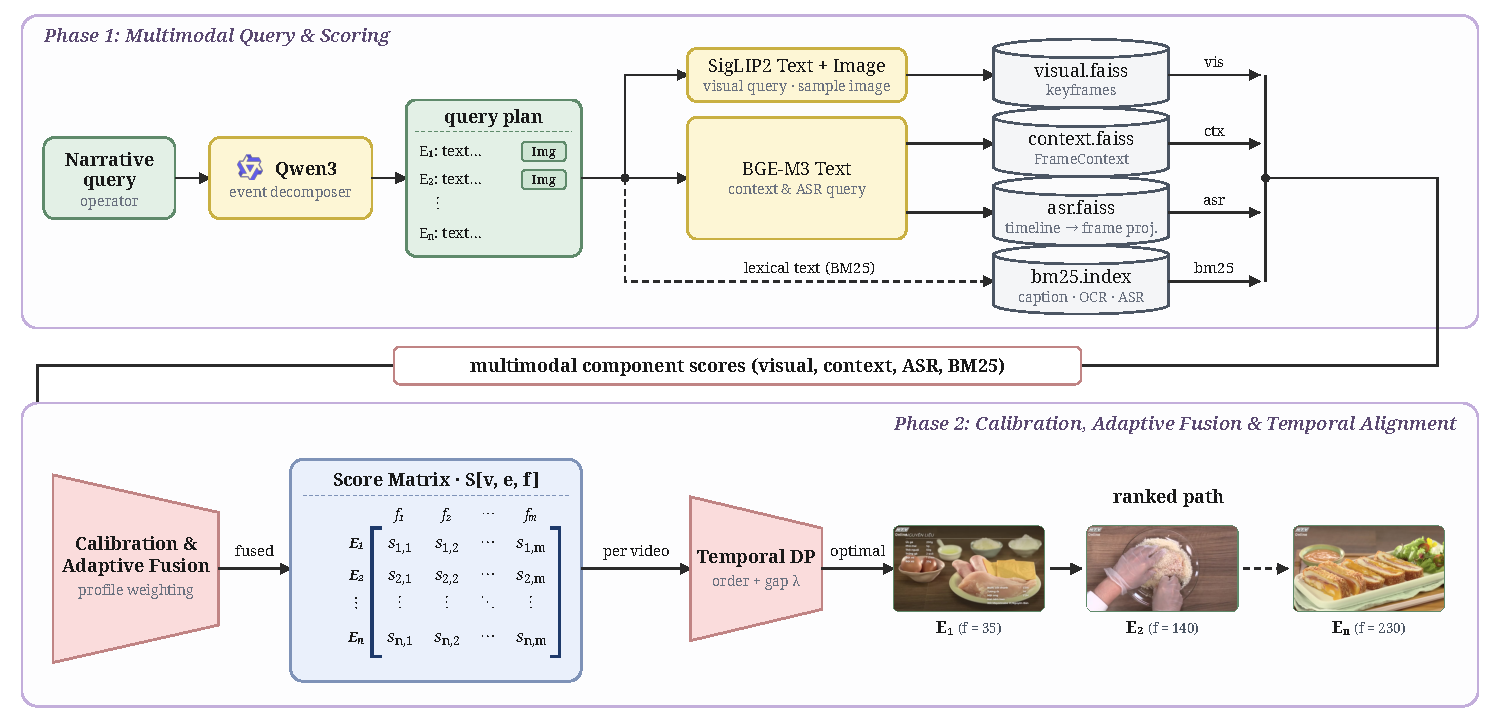
\includegraphics[width=0.82\textwidth]{layer2.pdf}
  \caption{Multi-event KIS retrieval pipeline in SHI. The Query Hypothesis
  provides an ordered sequence of events. Text events query visual,
  FrameContext, ASR, and lexical indexes, while optional reference images
  contribute visual similarity scores. Component scores are calibrated and
  fused into an event--frame score matrix $S[v,e,f]$ for each candidate video
  $v$. A dynamic-programming decoder then extracts chronologically ordered
  event paths, which are used to rank candidate videos and construct the
  evidence snapshot.}
  \label{fig:layer2}
\end{figure}

\subsection{Multi-event KIS Retrieval Pipeline}
\label{sec:kis-retrieval}

Multi-event KIS is formulated as multimodal event scoring followed by joint
temporal alignment. Given an ordered sequence of events from the Query
Hypothesis, each textual event is evaluated against several retrieval sources:
SigLIP2~\cite{tschannen2025siglip2} provides visual text--frame similarity,
BGE-M3~\cite{chen2024bgem3} provides dense FrameContext and ASR evidence, and
BM25~\cite{robertson2009bm25} provides lexical matching over frame-associated
text. Optional reference images contribute additional
SigLIP2 image--frame similarity scores. The resulting components are calibrated
and combined by event-adaptive weighted fusion into an event--frame score
matrix $S[v,e,f]$ for each candidate video $v$. A dynamic-programming decoder
then selects one canonical frame occurrence for each event subject to strict
temporal ordering. Its objective combines the fused event--frame scores with a
temporal gap penalty that discourages large separations between consecutive
event occurrences. Candidate videos are ranked by the scores of their decoded
paths, so the ranking accounts jointly for event-level evidence and temporal
ordering rather than aggregating independently selected frame matches.

\subsection{Evidence Snapshots and Competition Integration}
\label{sec:evidence-snapshots}

To support post-retrieval interaction without repeating corpus-level search,
SHI captures an in-memory \emph{Evidence Snapshot} after the initial KIS
execution. For the returned candidates, the snapshot retains immutable
event--frame evidence together with the event identifiers, initial decoded
paths, and the decoder configuration used for that search. When an operator
applies an EventTrail action, such as anchoring an accepted occurrence or
rejecting a temporal region, the corresponding constraints are maintained
separately from the frozen evidence and supplied to the temporal decoder. The
decoder then re-computes the feasible path for the selected video using the
retained evidence, without repeating query embedding or corpus index search.
Once the operator selects a frame for submission, SHI's integrated competition
client converts the selection to the required submission format and sends it
to the Distributed Retrieval Evaluation Server
(DRES)~\cite{rossetto2021dres}, reducing the need for manual transfer of frame
coordinates during live search.
\section{Interactive Hypothesis Correction}
\label{sec:interactive-hypothesis-correction}

SHI exposes two intermediate decisions in multi-event retrieval as explicit
interaction objects. Before retrieval, the \emph{Query Hypothesis} represents
how the input narrative has been interpreted as an ordered event sequence.
After retrieval, \emph{EventTrail} exposes how those events have been aligned
to occurrences within a selected video. Both representations can be inspected
before the user commits a correction.

\begin{figure*}[t]
    \centering
    % \includegraphics[width=\textwidth]{002_hypothesis_interaction.png}
    \fbox{\parbox[c][3.0cm][c]{0.96\linewidth}{\centering
    Hypothesis Interaction figure placeholder}}
    \caption{The two hypothesis-level interactions in SHI.
    \textbf{(a)} Query Hypothesis exposes the inferred event decomposition
    before retrieval and supports direct structural correction.
    \textbf{(b)} EventTrail exposes the decoded temporal hypothesis of a
    retrieved video and previews complete-path alternatives before a correction
    is committed.}
    \label{fig:hypothesis-interaction}
\end{figure*}

\subsection{Query Hypothesis}
\label{sec:query-hypothesis}

Interactive video retrieval systems commonly support query reformulation,
including suggestions derived from intermediate search results and
conversational refinement with relevance feedback
~\cite{lokoc2023queryreformulation,khan2024exquisitor,sharma2025exquisitor}.
Structured interfaces have also been used to express complex and temporal
queries~\cite{wu2021sql,heller2022temporalqueries}. SHI differs in the object
being edited: the system-generated interpretation of the original narrative is
itself exposed as a persistent \emph{Query Hypothesis} before retrieval.

For a multi-event request, SHI constructs an ordered sequence
\[
H_q=(E_1,E_2,\ldots,E_N),
\]
where each automatically generated event is grounded to a verbatim span of the
original query. The original request and its inferred event sequence are shown
together, allowing the user to inspect whether the decomposition preserves the
intended semantic and temporal structure.

Figure~\ref{fig:hypothesis-interaction}(a) shows the Query Hypothesis editor.
Users can edit an event, split it, merge adjacent events, change event order,
or add a new event. Image examples can additionally be associated with
individual events. In contrast to reformulating a single text query and
observing the resulting ranking, these operations directly modify the event
structure that will be used by the downstream retrieval and temporal-alignment
stages.

Edits are previewed before they affect the active hypothesis. The interface
shows the current and proposed event sequences side by side, after which the
user may cancel or apply the modification. Applying a change creates a new
query revision and marks results from the previous revision as outdated; a new
search is started explicitly by the user. Previous revisions can also be
restored through undo. This separates inspection and correction of the query
interpretation from search execution.

\subsection{EventTrail}
\label{sec:event-trail}

Prior systems support temporal query formulation and retrieval over sequences
or temporally related search conditions
~\cite{heller2021explainable,heller2022temporalqueries,khan2026temporalqueries}.
EventTrail instead exposes the \emph{decoded temporal hypothesis} of an
individual retrieved video: the current assignment of each query event to a
specific occurrence in that video.

Figure~\ref{fig:hypothesis-interaction}(b) presents this hypothesis as an
ordered event path, with each event associated with its selected frame and
timestamp. The user can focus on any event and inspect temporally distinct
alternative occurrences under the current constraints.

A central distinction of EventTrail is that an alternative is not presented as
an isolated frame. For each candidate occurrence of the focused event, SHI
decodes a complete chronologically valid path for the entire event sequence.
The user can therefore preview the consequence of selecting an alternative
before changing the active hypothesis. If other event assignments must move to
preserve chronological consistency, those changes are shown together with the
previewed path.

Previewing is non-mutating. The user can \emph{Keep} the current occurrence,
\emph{Use} a previewed alternative, or \emph{Reject} an incorrect temporal
mode. Keeping or using an occurrence introduces an anchor for that event,
whereas rejection excludes the corresponding temporal region. The complete
path is then re-decoded under the updated constraints using the multimodal
evidence retained from the original search.

Because temporal alignment is solved jointly for the complete event sequence,
a local correction may alter assignments of other events. EventTrail makes
these induced changes visible rather than treating each event match
independently. The interaction can be repeated across events, and previous
corrections can be undone when necessary.
\section{Conclusion}
\label{sec:conclusion}

We presented \textbf{SHI}, an interactive multimodal video retrieval system for
multi-event Known-Item Search at VBS 2027. SHI exposes two intermediate
retrieval hypotheses for direct user interaction. The pre-retrieval
\emph{Query Hypothesis} represents the LLM-generated event decomposition as an
editable ordered sequence, allowing operators to inspect and revise the search
structure before retrieval. The post-retrieval \emph{EventTrail} exposes the
decoded temporal alignment of an individual candidate video and supports
occurrence-level correction through anchor and exclusion constraints. By
retaining event--frame evidence in session-scoped Evidence Snapshots, SHI can
re-decode a constrained candidate path without repeating corpus-level
retrieval. Together, these mechanisms make semantic decomposition before
retrieval and temporal alignment after retrieval explicit interaction points
in the multi-event search workflow.
% % !TeX root = ../main.tex
\begin{credits}
\subsubsection{\ackname}
The authors thank the Video Browser Showdown organizers for organizing the
competition and maintaining its evaluation infrastructure.

\subsubsection{Disclosure of AI Assistance.}
During the preparation of this manuscript, the authors used AI-assisted tools
for language editing, phrasing refinement, and feedback on manuscript
organization and presentation. All scientific ideas, system designs,
implementation decisions, technical claims, and final manuscript content were
reviewed and approved by the authors, who take full responsibility for the
publication.
\end{credits}


\makeatletter
\renewenvironment{thebibliography}[1]
     {\section*{\refname}
      \def\@biblabel##1{##1.}
      \fontsize{8.5pt}{10.2pt}\selectfont
      \list{\@biblabel{\@arabic\c@enumiv}}%
           {\settowidth\labelwidth{\@biblabel{#1}}%
            \leftmargin\labelwidth
            \advance\leftmargin\labelsep
            \setlength{\itemsep}{-1.5pt}%
            \setlength{\parsep}{0pt}%
            \usecounter{enumiv}%
            \let\p@enumiv\@empty
            \renewcommand\theenumiv{\@arabic\c@enumiv}}%
      \renewcommand\newblock{\hskip .11em \@plus.33em \@minus.07em}%
      \sloppy\clubpenalty4000\widowpenalty4000%
      \sfcode`\.=\@m}
     {\def\@noitemerr
       {\@latex@warning{Empty `thebibliography' environment}}%
      \endlist}
\makeatother

\bibliographystyle{splncs04}
\bibliography{references}

\end{document}
